Seguindo para a última das arquiteturas de CNNs exploradas neste trabalho, temos a Inception-V3. Como na CNN anterior, foi treinado apenas um modelo com a abordagem B, a qual se aplicam as mesmas justificativas para tal.

Os hiperparâmetros, definidos de forma arbitrária, e as métricas obtidas para este modelo encontram-se na Tabela \ref{tab:inception}. Uma visualização da \emph{loss} e acurácia durante o treinamento estão caracterizados na Figura \ref{fig:treinamento-inception}.

\begin{table}[h!]
\centering
\caption{Detalhamento do modelo obtido com a arquitetura Inception-V3 para a abordagem B.}
\label{tab:inception}
\begin{tabular}{cccccc}
\toprule
\textbf{Otimizador} & \textbf{\emph{Patience}}  & \textbf{Função de Ativação} & \textbf{Acurácia} & \textbf{F-Score} & \textbf{EER} \\
\midrule
RMSprop & 5 & ELU & $0.8394$ & $0.8070$ & $16.9493$ \\
\bottomrule
\end{tabular}
\end{table}

\begin{figure}[H]
\centering
\caption{Histórico de \emph{loss} e acurácia durante o treinamento do modelo obtido com a arquitetura Inception-V3.}
\label{fig:treinamento-inception}
\subfloat[\emph{Loss} durante treinamento da rede Inception-V3 para a abordagem B.\label{subfig:inception-b-loss}]{%
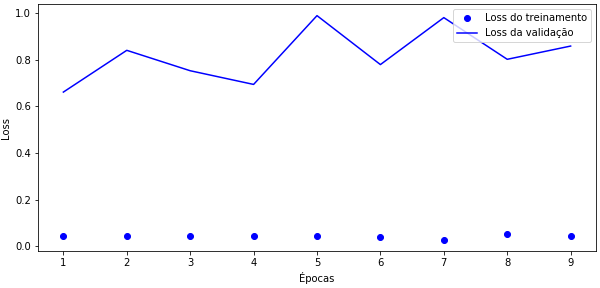
\includegraphics[width=0.47\textwidth]{imgs/inception-b-loss}
}
\hfill
\subfloat[Acurácia durante treinamento da rede Inception-V3 para a abordagem B.\label{subfig:inception-b-acc}]{%
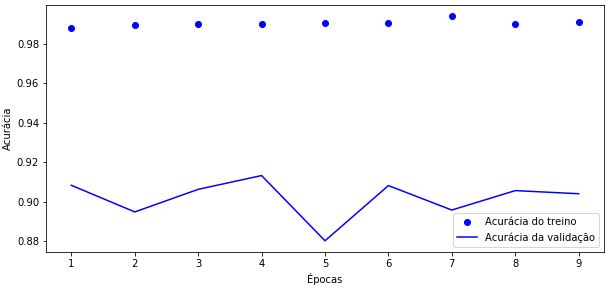
\includegraphics[width=0.47\textwidth]{imgs/inception-b-acc}
}
\end{figure}

É possível examinar a parada precoce do treinamento, levando apenas $9$ épocas antes de chegar ao final. Isto se deve, provavelmente, à capacidade da Inception de detectar os padrões das imagens, o que pode levar a um \emph{overfitting} ao conjunto de treinamento que, consequentemente, diminui o valor da acurácia no conjunto de validação.

A matriz de confusão exibida na Figura \ref{fig:matrizes-inception} diz respeito ao modelo treinado com esta arquitetura. Tem-se um resultado similar ao observado na arquitetura VGG-16, portanto, cabem aqui as mesmas ponderações demonstradas anteriormente.

\begin{figure}[h]
    \centering
    \caption{Matriz de confusão do modelo obtido com a arquitetura Inception-V3.}\label{fig:matrizes-inception}
    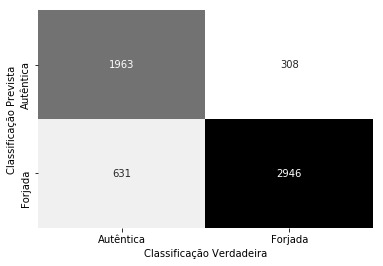
\includegraphics[width=0.6\textwidth]{imgs/matriz-inception}
\end{figure}

Por fim, foi possível comprovar que esta arquitetura consegue prestigiar nosso problema com resultados satisfatórios. Porém, novamente, fica aberta a reflexão sobre a necessidade da utilização de uma arquitetura tão profunda para tratar um problema que foi adequadamente ajustado por CNNs mais rasas. Não obstante, pode ser realizada uma busca exploratória sobre os hiperparâmetros, com vistas à descoberta de resultados superiores aos observados nestas arquiteturas rasas.